\section{Background}
In the context of the finite element response history analysis, seismic action can be introduced into the system via either force or deformation. For the former, acceleration record is converted to inertial force with the assist of mass and then applied to target degrees of freedom. For the latter, displacement record can be directly applied to supports to shake the structure as if it sits on a shaking table.
The typical sampling rate of ground motion seismograms ranges from \SI{50}{\hertz} to \SI{200}{\hertz}. This corresponds to a sampling period $T_s$ from \SI{5}{\milli\second} to \SI{20}{\milli\second}. Often such a time step size is not sufficient for non-linear response history analysis due to convergence issues. Ideally, the continuous--time version needs to be reconstructed from the discrete--time version of input seismogram in order to allow a smaller time step size to be used for simulation. However, it is obvious that the exact reconstruction is not achievable.

It is then a convention to perform linear interpolation between two adjacent discrete samples for the case that time step size (of numerical analysis) is different from sampling interval (of input seismogram). Essentially, the linear interpolation is equivalent to a low--pass finite impulse response (FIR) filter with a triangular window.

For the ease of discussion, let sampling interval be the multiple of time step size and let the ratio be $L$, which is an integer. It is then equivalent to upsample the input seismogram by the same ratio $L$. If the sampling rate/frequency of the original seismogram is $f_s$, then the upsampled signal has a sampling rate of $Lf_s$. Extra attention shall be paid to the original Nyquist frequency $f_s/2$ since anything above it cannot be reconstructed. For a discrete--time signal $p[n]$, a typical upsampling operation with upsampling factor $L$ consists of two steps:
\begin{enumerate}
\item Insert $L-1$ zeros between each pair of adjacent samples in $p[n]$, resulting in a new signal $p_e[n]$ which can be formally defined as
\begin{gather}
p_e[n]=\left\{
\begin{array}{ll}
p[n/L],&n=0,~L,~2L,~3L,~\cdots,\\
0,&\text{otherwise}.
\end{array}
\right.
\end{gather}
This is known as an expander, and is often denoted by $\uparrow{}L$ such that $p_e[n]=[\uparrow{}L]p[n]$.
\item Apply a low--pass filter with kernel $h[n]$ on $p_e[n]$ via convolution. The linear interpolation corresponds to the following kernel.
\begin{gather}
h[n]=\left\{
\begin{array}{ll}
1-\abs{n}/L,&\abs{n}\leqslant{}L-1,\\
0,&\text{otherwise}.
\end{array}
\right.
\end{gather}
The convoluted/interpolated/filtered signal is denoted as $p_i[n]$. In this work, different kernels will be discussed.
\end{enumerate}

Since the extended discrete signal $p_e[n]$ is $p[n]$ with additional zero samples, once the upsampling factor $L$ is chosen, $p[n]$ can be converted to $p_e[n]$ and vice versa. We focus on the properties of $p_e[n]$.

The bare $p_e[n]$ without applying any filters contains spectral images, that is, extra copies of the original spectrum $\omega\in[0,~f_s/2]$ in additional frequency domain $\omega\in[f_s/2,~Lf_s/2]$. For example, consider the sinusoid
\begin{gather}
u(t)=\sin\left(2\pi{}f_0t\right),
\end{gather}
with the frequency $f_0=\dfrac{\omega_0}{2\pi}$ chosen to be \SI{25}{\hertz}. Assume this continuous--time signal is sampled at rate $f_s=\SI{200}{\hertz}$, the discrete--time signal $p[n]$ can be depicted in \figref{fig:original}.
\begin{figure}[H]
\centering
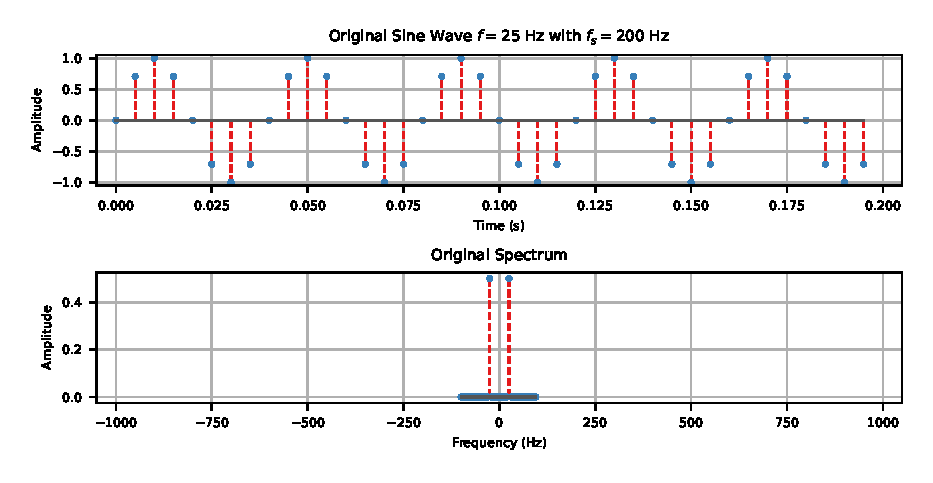
\includegraphics{PIC/PureSineOrigin}
\caption{original sine wave in time domain and frequency domain}\label{fig:original}
\end{figure}
The corresponding Nyquist frequency is $f_s/2=\SI{100}{\hertz}$, thus, the frequency ranges from \SI{-100}{\hertz} to \SI{100}{\hertz} (negative part not shown with amplitude properly scaled).

By choosing an upsampling factor $L=10$, the extended signal $p_e[n]$ (zero--stuffed) can be illustrated as in \figref{fig:extended}.
\begin{figure}[H]
\centering
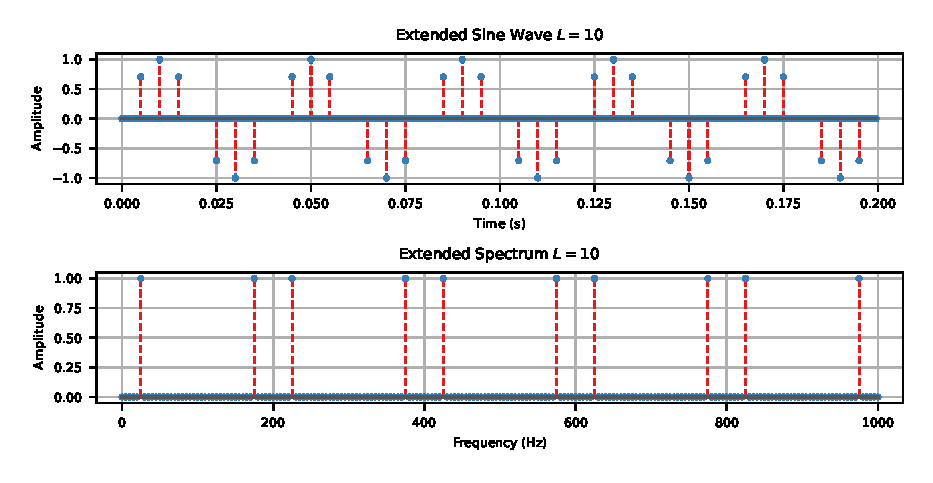
\includegraphics{PIC/PureSineExtended}
\caption{zero--stuffed sine wave in time domain and frequency domain}\label{fig:extended}
\end{figure}
The Nyquist frequency of $p_e[n]$ is $10\times\SI{100}{\hertz}=\SI{1000}{\hertz}$, the original component at $\SI{25}{\hertz}$ is copied in the additional frequency domain ranging from \SI{100}{\hertz} to \SI{1000}{\hertz}.

The linear interpolation (triangular window) can be constructed as
\begin{gather}
h[n]=0.1\times\begin{bmatrix}
1&2&3&\cdots&10&\cdots&3&2&1
\end{bmatrix},
\end{gather}
its frequency response can be seen in \figref{fig:tri_window}.
\begin{figure}[H]
\centering
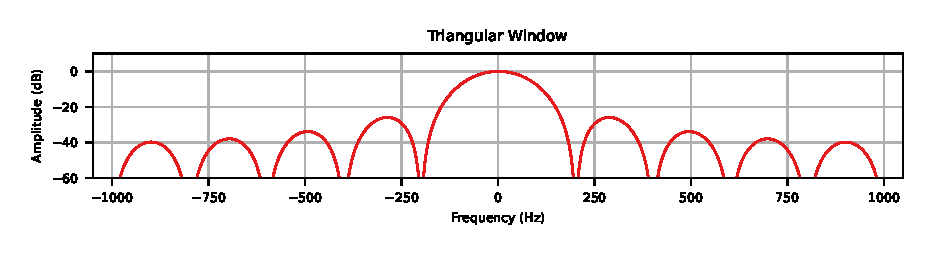
\includegraphics{PIC/TriangularWindow}
\caption{triangular window in frequency domain}\label{fig:tri_window}
\end{figure}

By the convolution theorem, the upsampled signal can be obtained by either performing the convolution in time domain or multiplication in frequency domain.
\begin{figure}[H]
\centering
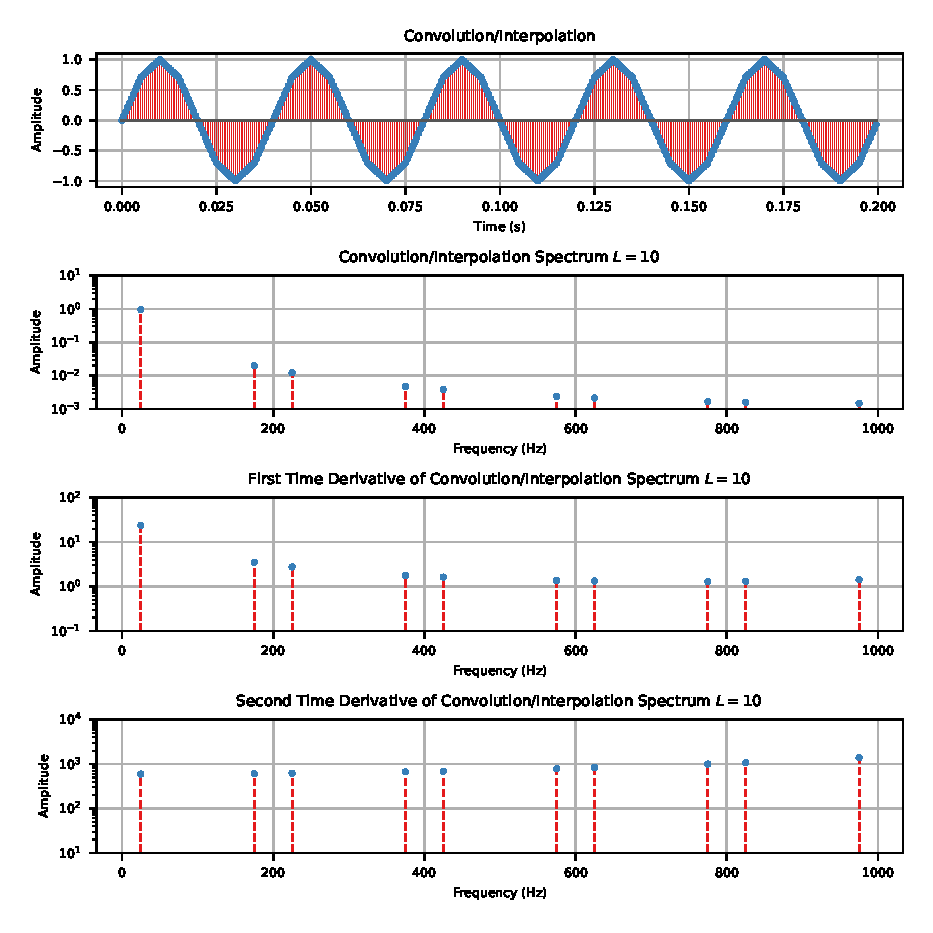
\includegraphics{PIC/Convolution}
\caption{interpolated sine wave in time domain and frequency domain}\label{fig:interpolated}
\end{figure}
\figref{fig:interpolated} shows the interpolated signal in both time domain and frequency domain. Due to the high side lobe level (around \SI{-26}{\decibel} of the first side lobe) of the triangular window, although the spectral images in $p_i[n]$ between \SI{100}{\hertz} and \SI{1000}{\hertz} are seemingly attenuated.

To investigate how the partially attenuated images would affect the response of an oscillator system, consider a single degree of freedom mass--spring--dashpot linear system under harmonic load. The equation of motion can be written as
\begin{gather}
ma\left(t\right)+cv\left(t\right)+ku\left(t\right)=p\left(t\right),
\end{gather}
with $p\left(t\right)=p_0\sin\left(2\pi{}ft\right)$ where $p_0$ is the amplitude of the harmonic, and its angular frequency is $\omega=2\pi{}f$.

Duhamel's integral shows the solution to this system can be expressed as
\begin{gather}\label{eq:duhamel}
u\left(t\right)=\int_{0}^{t}p\left(\tau\right)h\left(t-\tau\right)\md{\tau},
\end{gather}
with the fundamental solution
\begin{gather}
h\left(t\right)=\dfrac{1}{m\omega_d}\exp\left(-\zeta\omega_nt\right)\sin\left(\omega_dt\right),
\end{gather}
where $m$ is the mass, $c$ is the damping coefficient, $k$ is the stiffness, $\omega_n=\sqrt{\dfrac{k}{m}}$ is the natural frequency of the system, $\zeta=\dfrac{c}{2\sqrt{mk}}$ is the damping ratio, $\omega_d=\omega_n\sqrt{1-\zeta^2}$ is the damped frequency. The following discussion is confined within underdamped cases ($\zeta<1$).

\eqsref{eq:duhamel} can be conveniently evaluated in the frequency domain via Fourier transform, such that
\begin{gather}
\hat{u}\left(\omega\right)=\mathscr{F}\left\{u\left(t\right)\right\}=\mathscr{F}\left\{p\left(t\right)\right\}\cdot\mathscr{F}\left\{h\left(t\right)\right\}=\hat{p}\left(\omega\right)\cdot\hat{h}\left(\omega\right),
\end{gather}
with
\begin{gather}
\hat{h}\left(\omega\right)=\dfrac{1}{k}\dfrac{1}{\left(1-\beta^2\right)+i\left(2\zeta\beta\right)},\qquad\beta=\dfrac{\omega}{\omega_n}.
\end{gather}

The velocity spectrum can be obtained by differentiating $\hat{u}\left(\omega\right)$,
\begin{gather}
\hat{v}\left(\omega\right)=i\omega\cdot{}\hat{u}\left(\omega\right)=i\omega\cdot{}\hat{p}\left(\omega\right)\cdot\hat{h}\left(\omega\right).
\end{gather}

If the damping force is denoted by $F_d$, then it is possible to derive that
\begin{gather}
\hat{F_d}\left(\omega\right)=\mathscr{F}\left\{F_d\left(t\right)\right\}=c\cdot{}\hat{v}\left(\omega\right)=c\cdot{}i\omega\cdot{}\hat{p}\left(\omega\right)\cdot\hat{h}\left(\omega\right).
\end{gather}
We further denote
\begin{gather}
\hat{k}\left(\omega\right)=ic\omega\cdot\hat{h}\left(\omega\right),
\end{gather}
which links external load spectrum $\hat{p}\left(\omega\right)$ to the damping force spectrum $\hat{F_d}\left(\omega\right)$.

Now consider three different types of damping.
\paragraph{Constant Damping}
Let $c$ (and $\zeta$) be a constant, then
\begin{gather}
\hat{F_d}\left(\omega\right)=\hat{p}\left(\omega\right)\cdot\dfrac{i\left(2\zeta\beta\right)}{\left(1-\beta^2\right)+i\left(2\zeta\beta\right)}.
\end{gather}
\paragraph{Mass Proportional Damping}
Let $c$ be proportional to mass such that $c=2a_0m$, then
\begin{gather}
\zeta=\dfrac{2a_0m}{2\sqrt{mk}}=\dfrac{a_0}{\omega_n},\qquad
\zeta\beta=\dfrac{a_0\omega}{\omega_n^2},
\end{gather}
so that
\begin{gather}
\hat{F_d}\left(\omega\right)=\hat{p}\left(\omega\right)\cdot\dfrac{i\left(2a_0\omega\right)}{\left(\omega_n^2-\omega^2\right)+i\left(2a_0\omega\right)}.
\end{gather}
\paragraph{Stiffness Proportional Damping}
Let $c$ be proportional to stiffness such that $c=2a_1k$, then
\begin{gather}
\zeta=\dfrac{2a_1k}{2\sqrt{mk}}=a_1\omega_n,\qquad
\zeta\beta=a_1\omega,
\end{gather}
so that
\begin{gather}
\hat{F_d}\left(\omega\right)=\hat{p}\left(\omega\right)\cdot\dfrac{i\left(2a_1\omega\right)}{\left(1-\beta^2\right)+i\left(2a_1\omega\right)}.
\end{gather}

It can be noticed that all three expressions of $\hat{F_d}\left(\omega\right)$ possess a similar form
\begin{gather}
\hat{F_d}\left(\omega\right)=\dfrac{iA}{B+iA},
\end{gather}
and $B=0$ when $\omega=\omega_n$, where the maximum magnitude \num{1} is achieved. At this exact point, the magnitude of damping force component simply equals that of the external load component. The magnitude distribution of $\hat{k}\left(\omega\right)$ in frequency domain can be computed and illustrated in \figref{fig:constant_damping}, \figref{fig:k_proportional} and \figref{fig:m_proportional}.
\begin{figure}[H]
\centering
\includegraphics[]{PIC/ConstantProportional2000}
\caption{fundamental solution with constant damping}\label{fig:constant_damping}
\end{figure}

\begin{figure}[H]
\centering
\includegraphics{PIC/StiffnessProportional10}
\caption{fundamental solution with stiffness proportional damping}\label{fig:k_proportional}
\end{figure}

\begin{figure}[H]
\centering
\includegraphics{PIC/MassProportional500000}
\caption{fundamental solution with mass proportional damping}\label{fig:m_proportional}
\end{figure}